\chapter{Concept\label{cha:chapter4}}

Not only the requirements form the previous chapter \ref{cha:chapter3} but also the analysis and assessment of faulty data in \ref{cha:chapter2} is the basis for concept design of the resulting framework proposal. This chapter introduces the design of the overall framework and its components as well as its architectural design.

\section{Overall framework design \label{sec:overalldesign}}

\begin{figure}[htb]
  \centering
  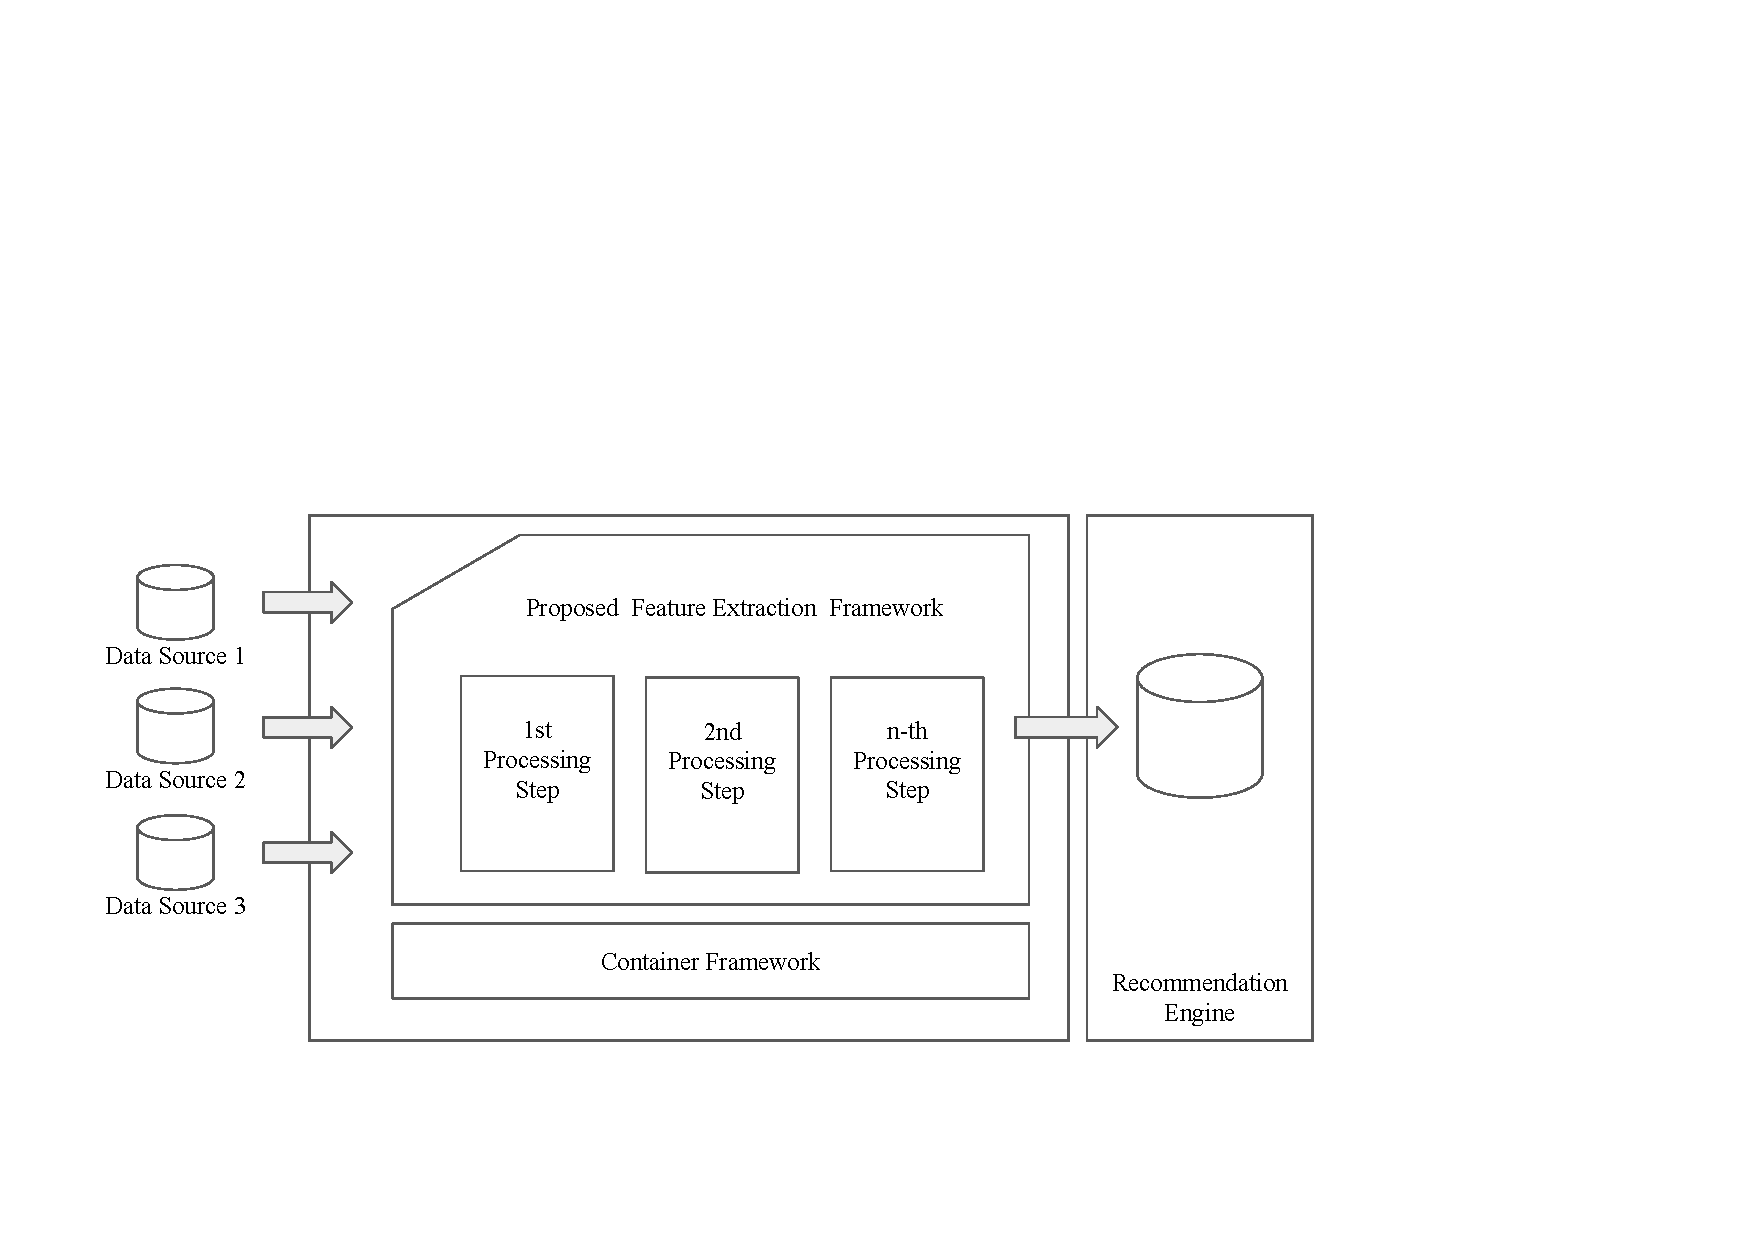
\includegraphics[width=0.9\textwidth]{concept-framework}\\
  \caption{Basic concept of feature extraction framework}
  \label{fig:basicconcept}
\end{figure}

To satisfy the requirements of simple adaptability and reliable system a modularized framework concept is applied. A pipelined approach with adaptable components characterizes the overall framework design. A software application of the proposed framework is desirable. Therefore, modularized software design and development ensures a level of abstraction that aims for simple update, exchange or addition of features. Single modules are implemented encapsulated and exchange data via APIs on different transportation technologies. Common data structures and interfaces are shared via libraries which are simply a further module of the framework. Namely \textit{core} or \textit{common} libraries in various software projects. Compare modules and components, also available as libraries, of the Apache Fink framework. % https://mvnrepository.com/artifact/org.apache.flink
\\\\
Revisiting the in chapter \ref{cha:chapter3} stated requirements leads to the breakdown of the framework into the following modules:
\begin{itemize}
\item Source adapters
\item Parsing pipeline
\item Output adapter
\item Error pipeline
\end{itemize}
In addition to handle underlying data transfer and processing a container framework is used. This simplifies the implementation of the feature extraction framework and abstracts the heavy lifting of data processing.
\\\\
The pipeline concept facilitates the handling of single and multiple source problems analyzed in chapter \ref{cha:chapter2}. A three step approach towards clean features is chosen to tackle structural problems and issues on entity level at once. Internally the framework must use a one data schema to reduce overhead on transformation as well as introduction of errors.

\section{Concept and use of the container framework \label{sec:containerframework}}

Many data processing frameworks are available nowadays. Especially the trend of big data emerged frameworks on different abstraction layers. Most of them have their foundations in widely known concept of Map Reduce or any of its descendants. Promising Open source examples in this case are among others Apache Flink, Apache Samza, Apace Spark or Kafak Streams. Conceptual the container framework hides away underlying data transportation and enables the use of user defined code and user defined functions. There the in the previous paragraph mentioned modules can introduced. This abstract concept will allow to exchange the underlying container framework as well as consecutive modules. In the next chapter, chapter \ref{cha:chapter5}, after evaluation of different container frameworks the best suitable is determined.

\section{Concept of the input adapter \label{sec:inputadapter}}

The input adapters are mainly responsible for format and schema specific generalization of incoming data. The drawbacks of heterogeneous file formats is covered in section \ref{sec:stateanalysis}. From this we know it is essential to find a common and flexible way to represent data within one system. The concepts does not make any suggestions regarding the format to be chosen, as the framework must not rely on implementation specifications. It only suggests that one common schema for the entire framework to avoid translation overhead and internal error sources. For a generalization purpose the concept defines a library which enables an easy adaption to multiple data sources, their formats and schemas. The formats can be found on the y-axis in figure \ref{fig:inputadapter}. As we speak about data unification in this work, on the other axis the raw entity type can be found. For instance, if the features for animal entities have to be found across different sources the library provides a tool set to define as the input format and the output schema. Furthermore the input adapter provides the functionality to combine a specific input source with a specific output entity an an abstract level. In a concrete case the developer must have a interface provided to define the source depended schema and a user defined function (UDF)\footnote{A UDF is a function that is executed in a bigger context, accepts parameters performs non-side-effecting transformation and returns the result} to map between source schema and the raw target schema. Additional source depended knowledge can be applied on the data. For instance, internal quantities and units can be transformed to international standards. The concept defines a library which plugs in a custom source schema on a predefined (or custom) data source, mapping function to translate the source schema and the definition of the raw target schema. The UDF has a very simple interface, as it is defined as a function mapping a source custom source schema to a raw target schema. The raw schema does not support deterministic values but defines a set of attributes necessary for further processing steps.

\begin{figure}[htb]
  \centering
  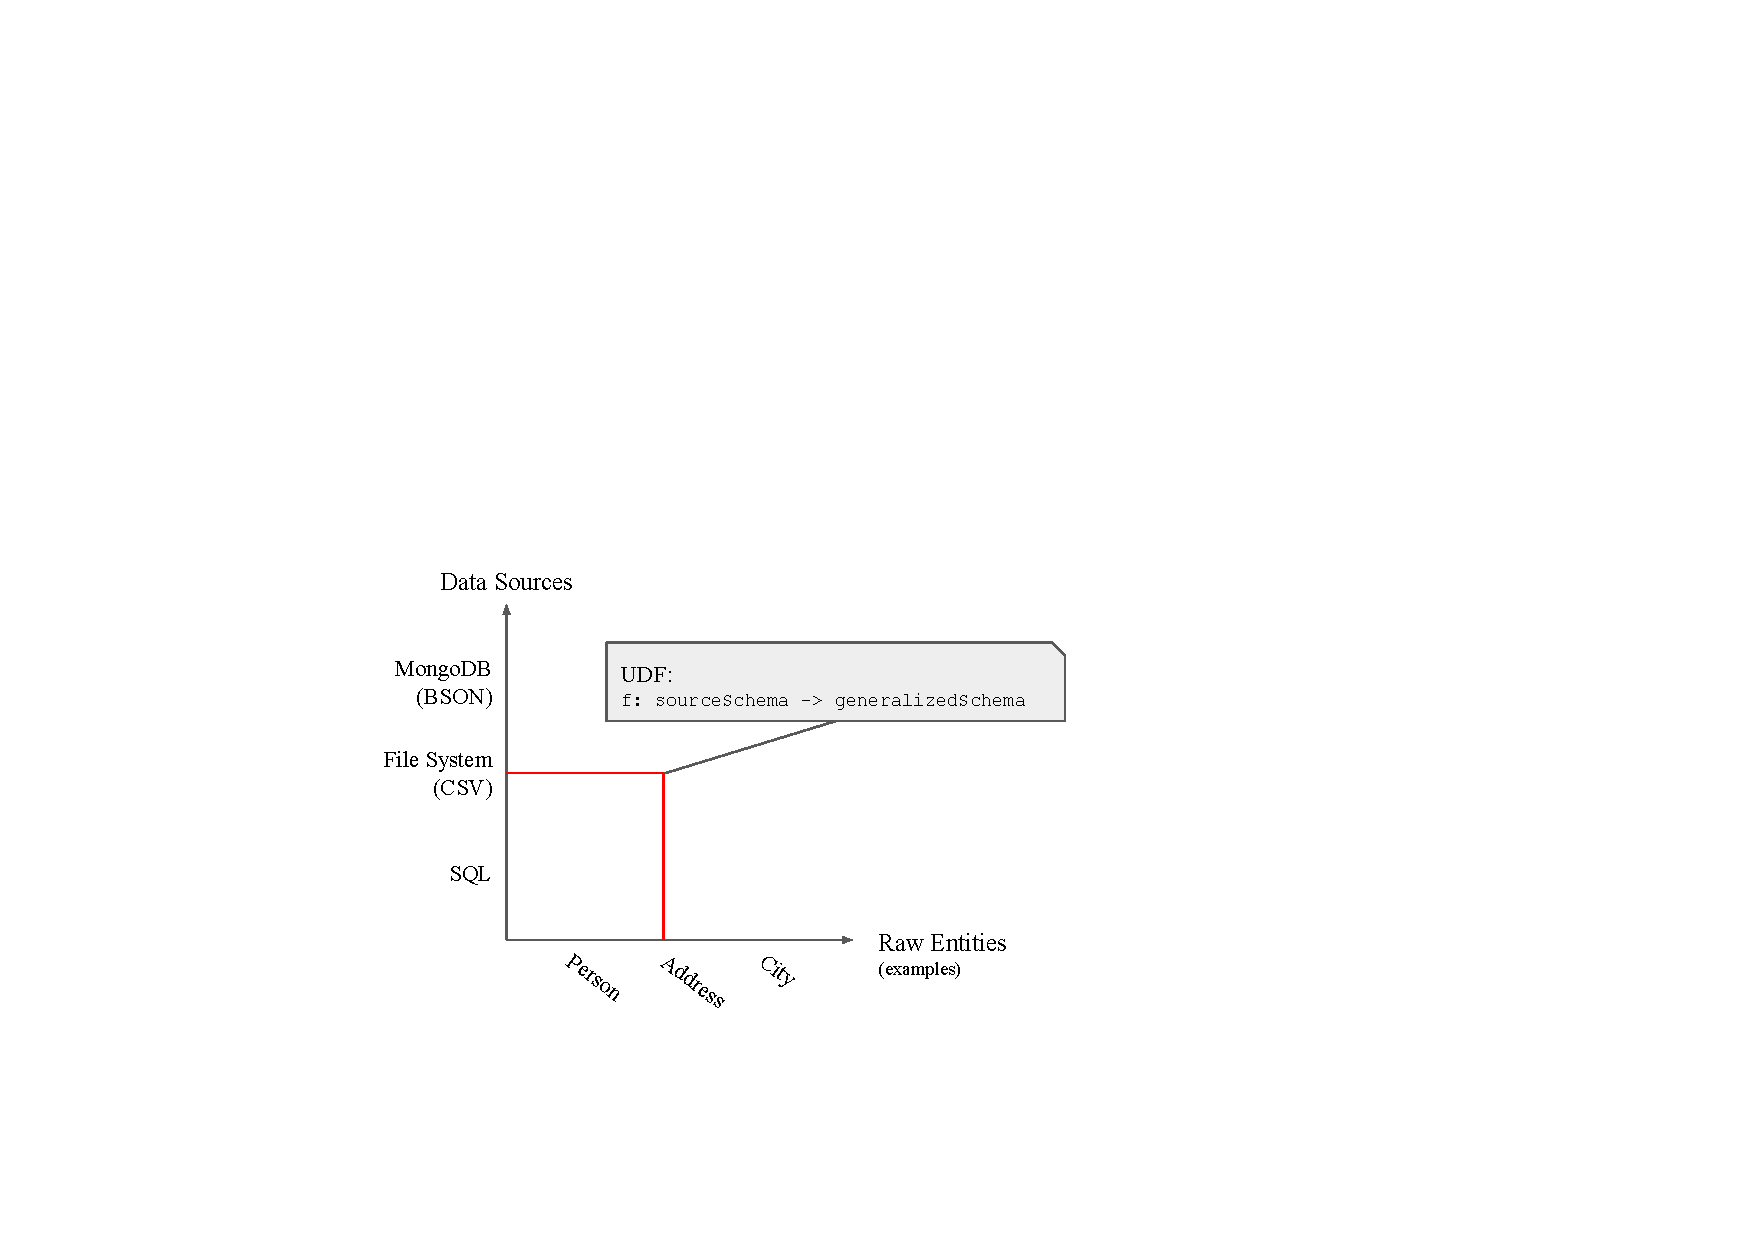
\includegraphics[width=0.6\textwidth]{input-adapter}\\
  \caption{Concept of input adapter library}
  \label{fig:inputadapter}
\end{figure}

\section{Concept of parsing pipeline}

The core of the processing framework is the centralized parsing pipeline. At this point the raw schema is transfered to a generalized schema. The difference here is that the raw schema can be considered as stable and therefore adequate transformation can be applied. The concept suggests that the transformation is split up in different steps which perform different types of computations on the respective raw entity. The generalized schema is to be provided by a developer but is committed on domain level in which the proposed framework is operating. As already explained in the previous section, section \ref{sec:inputadapter}, the concept of UDFs provides a flexible method of introducing custom functionality into a predefined system. For the parsing pipeline the same approach is applicable, as the raw entity is transformed over a deterministic number of steps towards a generalized schema. 
\\\\
Possible parsing steps among others are:
\begin{itemize}
\item Unification of different levels of normalization
\item Source independent transformation
\item Homogenization of attribute value manifestations
\end{itemize}

The abstraction of an parsing step must allow the connection to a second data source for potential data enrichment through lookups. Another obligatory feature is a initial loading of a user defined resource such as a mapping table or a model. For this type of application of the processing pipeline a asynchronous processing should be possible to avoid a blocking of the pipeline.

\section{Concept of pluggable output adapters}

The pluggable output adapters are meant for further transformations of the generalized entity that results from the parsing pipeline. Based of different intents of using the homogenized data, a set of outputs is desired. This boils down to data formats that are required by the acutaly application downstream of the feature extraction framework. From a framework aspect the output adapter is similar to the input adapters. The concept differs in a deterministic input as well as output schema or a set of deterministic schemas, depending on the post-processing use cases. The input schema is analog to the final output schema of the parsing pipeline and due to the fact of a unified format within the overall framework does not produce additional development overhead. 

\section{Concept of error pipeline \label{sec:errorpipeline}}

From the requirements (chapter \ref{cha:chapter3}, section \ref{sec:error}) a concept for error persistence and processing guarantees is developed. The overview in figure \ref{fig:basicconcept} show a component called \textit{Error Pipeline}. The idea of the error pipeline is to create a bypass stream of faulty data. Faulty data are defined by the fact that they could not processed in any steps of the framework. Faulty data from different steps of processing must be marked with the kind of error and the step where the error occurred. This must be done manly for a administrative purpose and manual quality check. Therefor the data can be located in different streams or data collections from where they can be fetched to analyze the underlying problem.

\section{Concept of quality assurance and ability of administration}

The quality assurance component of the automated framework is and overreaching element. Already lined out in section \ref{sec:errorpipeline}, occurring errors need to be handled. Other tasks to perform from an quality aspect are the control of the ongoing learn process of the entire system. Configuration of parsing rules and updating of mapping references are features to be controlled through an admin interface. For that, the system needs to be defined such that on different entry points over the modules interactions can take place. This is special for the parsing pipeline. As already explained, singular steps are configurable from the outside. The concept defines a dedicated interference point such as a database or data storage. Furthermore the injection of of quality concerns right after parsing but before sending data downstream through the output adapters is implemented. Manual crosschecks through an interface are enable. Additionally the manual introduction of generalized data satisfies the need for the required processing guarantees. 